\documentclass[a4paper, 12pt]{article}
\usepackage[utf8]{inputenc}
\usepackage{graphicx}
\usepackage{subcaption}
\usepackage{float}
\usepackage{amsmath}
\usepackage{amssymb}
\usepackage{lipsum}
\usepackage{hyperref}
\setlength{\belowcaptionskip}{-10pt}
\DeclareMathSizes{10}{12}{12}{12}
\usepackage[margin=0.8in]{geometry}
\usepackage{color} %red, green, blue, yellow, cyan, magenta, black, white
\definecolor{mygreen}{RGB}{28,172,0} % color values Red, Green, Blue
\definecolor{mylilas}{RGB}{170,55,241}
\usepackage{listings}
\lstset{escapeinside={<@}{@>}}
\usepackage{cite}
\usepackage{url}
\usepackage{tikz}
\usepackage{booktabs}
\usetikzlibrary{automata, positioning}
\usepackage{fancyheadings}
\usepackage{dsfont}
\usepackage{mathrsfs}
\usepackage{afterpage}
\usepackage{physics}

\newenvironment{changemargin}[2]{%
\begin{list}{}{%
\setlength{\topsep}{0pt}%
\setlength{\leftmargin}{#1}%
\setlength{\rightmargin}{#2}%
\setlength{\listparindent}{\parindent}%
\setlength{\itemindent}{\parindent}%
\setlength{\parsep}{\parskip}%
}%
\item[]}{\end{list}}
%useful tool for hiding stuff that breaks
\iffalse %(starts environment)
%(hidden stuff)
\fi % (ends environment)

\lstset{language=R,%
    basicstyle=\ttfamily,
	frame=none,
    framesep=19pt,
    breaklines=true,%
    belowskip=0.5cm,
    aboveskip=0.5cm,
    morekeywords={matlab2tikz},
    keywordstyle=\color{blue},%
    morekeywords=[2]{1}, keywordstyle=[2]{\color{black}},
    identifierstyle=\color{black},%
    stringstyle=\color{mylilas},
    commentstyle=\color{mygreen},%
    showstringspaces=false,%without this there will be a symbol in the places where there is a space
    numbers=none,
    numberstyle={\tiny \color{black}},% size of the numbers
    numbersep=9pt, % this defines how far the numbers are from the text
    emph=[1]{for,end,break},emphstyle=[1]\color{red}, %some words to emphasise
    %emph=[2]{word1,word2}, emphstyle=[2]{style},    
}


\begin{document}
\section*{Intro}

We wish to identify cells with mitochondrial dysfunction by the expression of proteins present. \\
We have frozen tissues from patients with mitochondrial disease and tissues from `healthy' subjects. The classification task utilises Bayesian linear regression to identify the relationship between the levels of protein expression within healthy subjects, then we again use Bayesian linear regression to find the relationship in patient samples, basing prior beliefs for the parameters on the posterior distributions from the control data. This allows us to calculate the proportion of deficient fibres. A fibre is considered deficient if it lies outside the error bounds of the regression line, the prior belief is that deficient fibres would not have a higher level of protein expression than a `healthy' subject. 

\section*{Previous Approach}
Before using a Bayesian methodology fibres were categorised as deficient if the protein expression level fell below the 95\% predictive interval of a linear model fitted using least squares. This can be seen in Figure \ref{fig:PlotsWithDots}. This did not allow for there to be differences between the control and patient data. 

\begin{figure}[H]
    \centering
    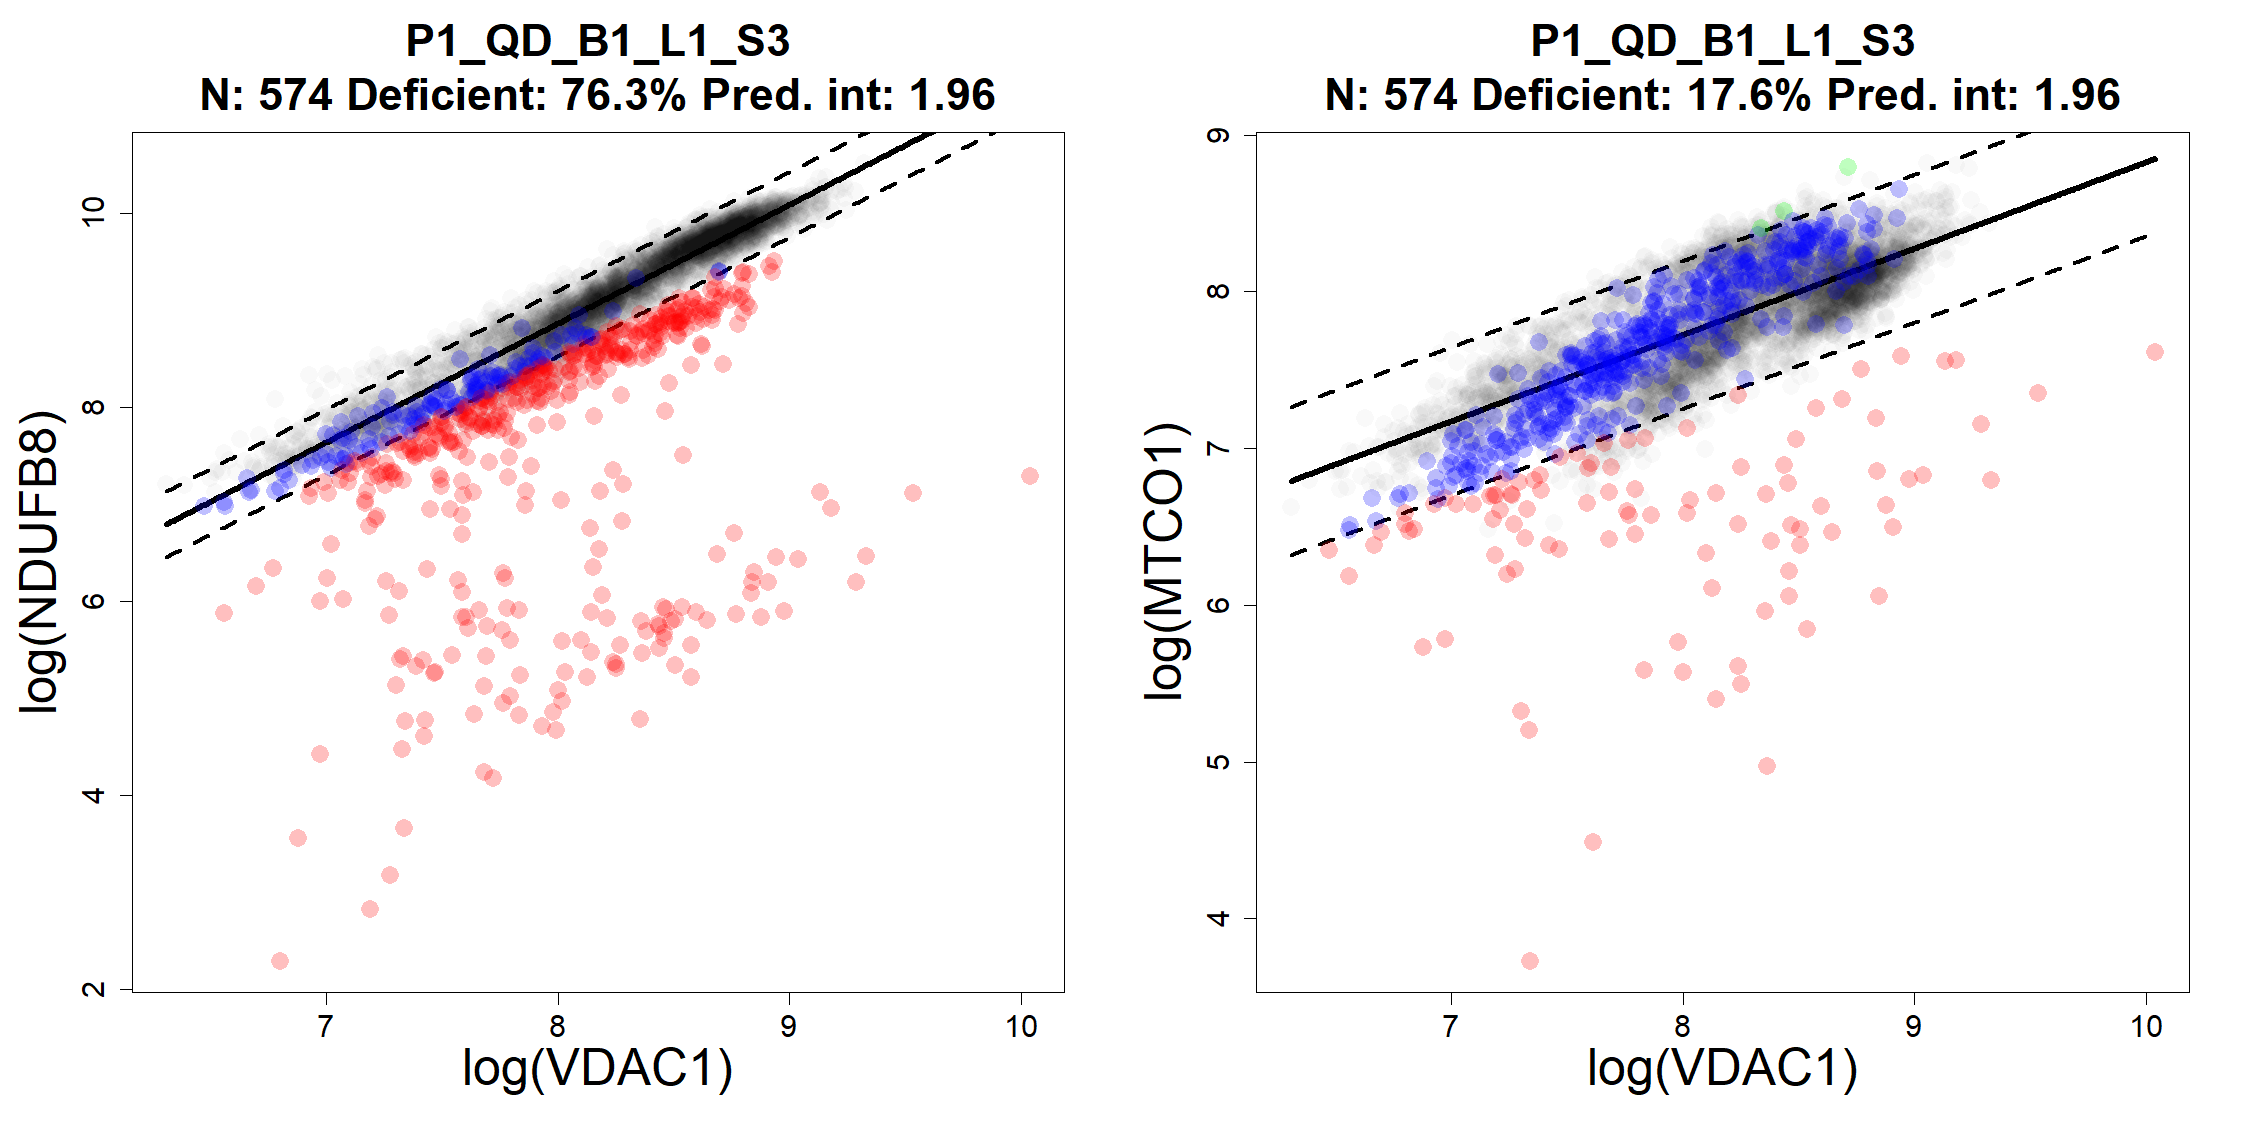
\includegraphics[width=0.8\textwidth]{freq_reg.png}
    \caption{Old model for categorising deficient fibres.}
    \label{fig:PlotsWithDots}
\end{figure}
Figure \ref{fig:StripByProt} shows the proportion of deficient fibres, in multiple samples from the same patient. A bootstrapping method was used to draw samples from this. 
\begin{figure}[H]
    \centering
    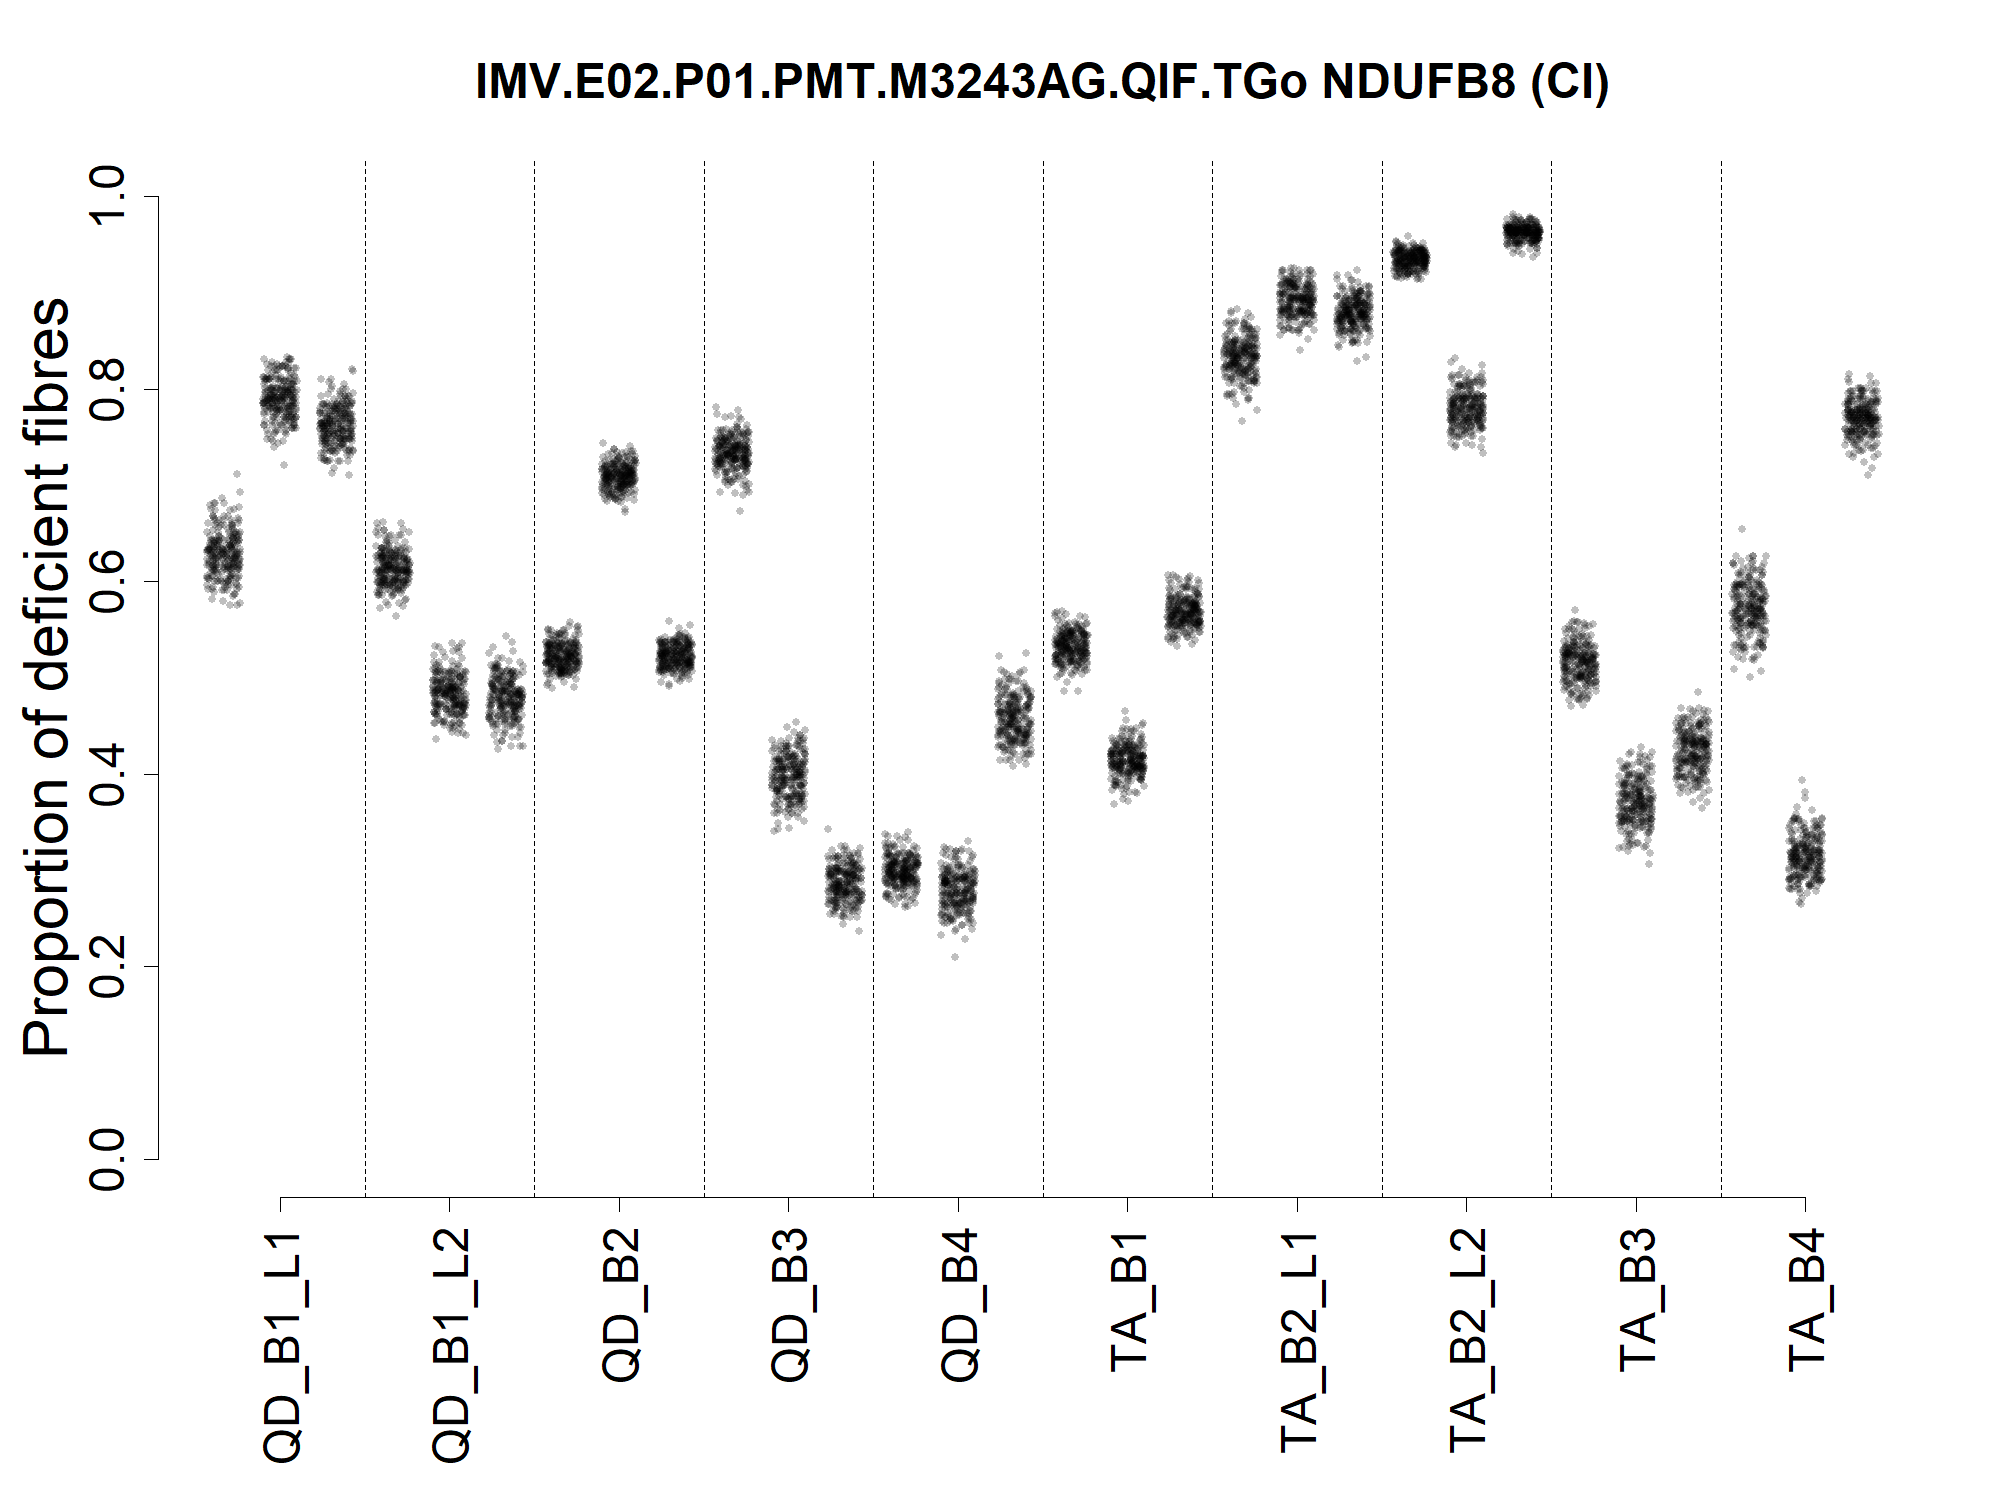
\includegraphics[width=0.5\textwidth]{freq_prop.png}
    \caption{Proportion of deficient fibres in a single patient, from different samples.}
    \label{fig:StripByProt}
\end{figure}


\section*{New Approach}

Let the response and explanatory variables be denoted as follows. 
\begin{center}
\begin{tabular}{ c | l }
    $Y_{obs}$ & the logged mass of NDUFB8, a protein coding gene linked to mitochondrial disease  \\
    \hline
    $X_{obs}$ & the logged mass of VDAC1, the most common antibody found on a mitochondrial membrane \\
\end{tabular}
\end{center}
We model the response variable, $Y_{obs}$, as
\begin{equation}
    Y_{obs} \sim \text{N}\left( m*X_{obs}+c, \hat\tau^{-1} \right).
\end{equation}
For the control data, from `healthy' cells, the parameters are given the following prior distributions:

\begin{minipage}{0.5\textwidth}
    \begin{itemize}
        \item[] $m\sim\text{N}\left(0, \hat{\tau}^{-1} \right)$ 
        \item[] $c\sim\text{N}\left(0, \hat{\tau}^{-1} \right)$
        \item[] $\tau \sim \text{Gamma}\left(2,2\right)$
    \end{itemize}
\end{minipage}
\begin{minipage}{0.5\textwidth}
    \begin{itemize}
        \item[] $\hat{\tau} = \begin{cases} \tau_{par},&\text{ if deficient }\\0.00001,&\text{ if control } \end{cases}$ 
        \item[] $\tau_{par} = \tau + \delta $
        \item[] $\delta =0 $
    \end{itemize}
\end{minipage}
The prior density for $\tau$ can be seen in Figure \ref{fig:tau_prior_ctrl}.
\begin{figure}[H]
    \centering
    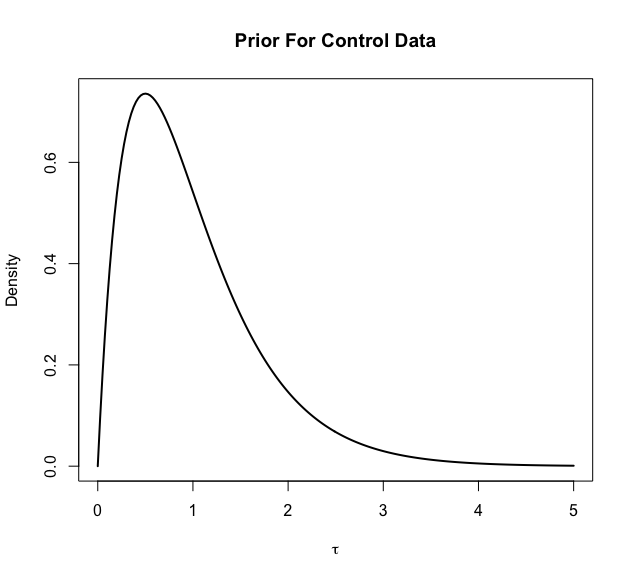
\includegraphics[width=0.5\textwidth]{tau_prior_ctrl.png}
    \caption{Prior density for $\tau$, control data.}
    \label{fig:tau_prior_ctrl}
\end{figure}
Here $\delta=0$ but the same form for the prior will be in given to the non-control data, where $\delta$ will be non-zero. The small precision for control data means that all fibres will be considered `healthy' as they will lie inside the 95\% error bounds. The model is written into RJAGS as the following:
\begin{lstlisting}
modelstring = "
 model {
  # Likelihood of data given model parameters
  for (i in 1:N){
   class[i] ~ dbin( probdiff, 1 )
   Yobs[i] ~ dnorm( Y[i], tau_hat[i] )
   Y[i] = m*Xobs[i] + c
   tau_hat[i] = ifelse( class[i]==0, tau_par, 0.00001 ) 
  }
  for (j in 1:Nsyn){
   Ysyn[j] ~ dnorm( Ys[j], tau_par )
   Ys[j] = m*Xsyn[j] + c
  }
  # Specify prior beliefs about parameters
  m ~ dnorm(mu_m,tau_m)
  c ~ dnorm(mu_c,tau_c)
  tau ~ dgamma(shape_tau,rate_tau)
  tau_par = tau + delta
  probdiff ~ dbeta(alpha,beta)  
 }
"
\end{lstlisting}

For non-control subjects, information gained during from the control dataset is used to determine prior beliefs. The prior means are set to the be the posterior means of the control data. The prior precision is the posterior precision multiplied by a scale factor. This results in a larger prior variance, so that to allow for difference between control data and patient data.\\ 

\begin{minipage}{0.5\textwidth}
    \begin{itemize}
        \item[] $m\sim \text{N}\left( \bar{m_c},\left[\frac{f}{sd(\boldsymbol{m}_c)^2}\right]^{-1}\right) $
        \item[] $c\sim\text{N}\left(\bar{c_c}, \left[\frac{f}{sd(\boldsymbol{c}_c)^2}\right]^{-1}\right) $
        \item[] $\tau\sim\text{Gamma}\left(2,5\right)$
    \end{itemize}
\end{minipage}
\begin{minipage}{0.5\textwidth}
    \begin{itemize}
        \item[] $\tau_{par} = \tau + \delta $
        \item[] $\delta = 1.5*\text{median}(\boldsymbol{\tau}_c)$
        \item[] $f=0.01$
    \end{itemize}
\end{minipage}

Where a subscript $c$ represents the draws from the posterior of the respective control variables posterior distribution and $ \bar{\cdot} $ represents the mean of the draws from the respective posterior distribution.\\

The prior density for $\tau$ can be seen in Figure \ref{fig:tau_prior_pat}.
\begin{figure}[H]
    \centering
    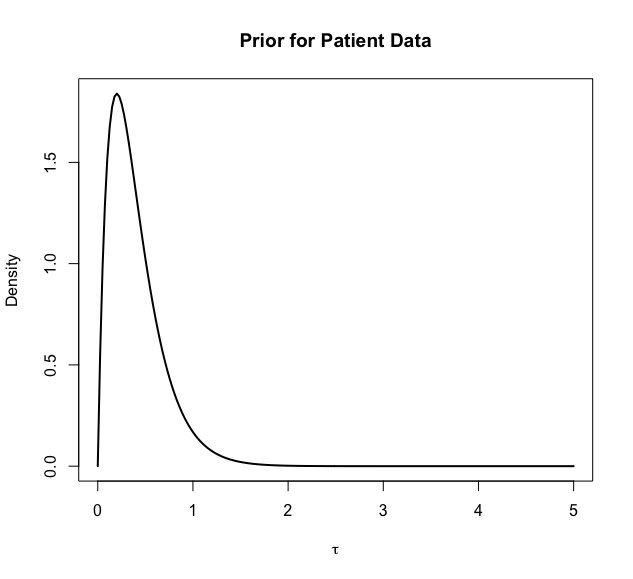
\includegraphics[width=0.5\textwidth]{tau_prior_pat.png}
    \caption{Prior density for $\tau$, for patient data.}
    \label{fig:tau_prior_pat}
\end{figure}

Figure \ref{fig:IMV} shows the proportion of deficient fibres in a single patient across multiple tissue samples, when using the Bayesian method. 

\begin{figure}[H]
    \centering
    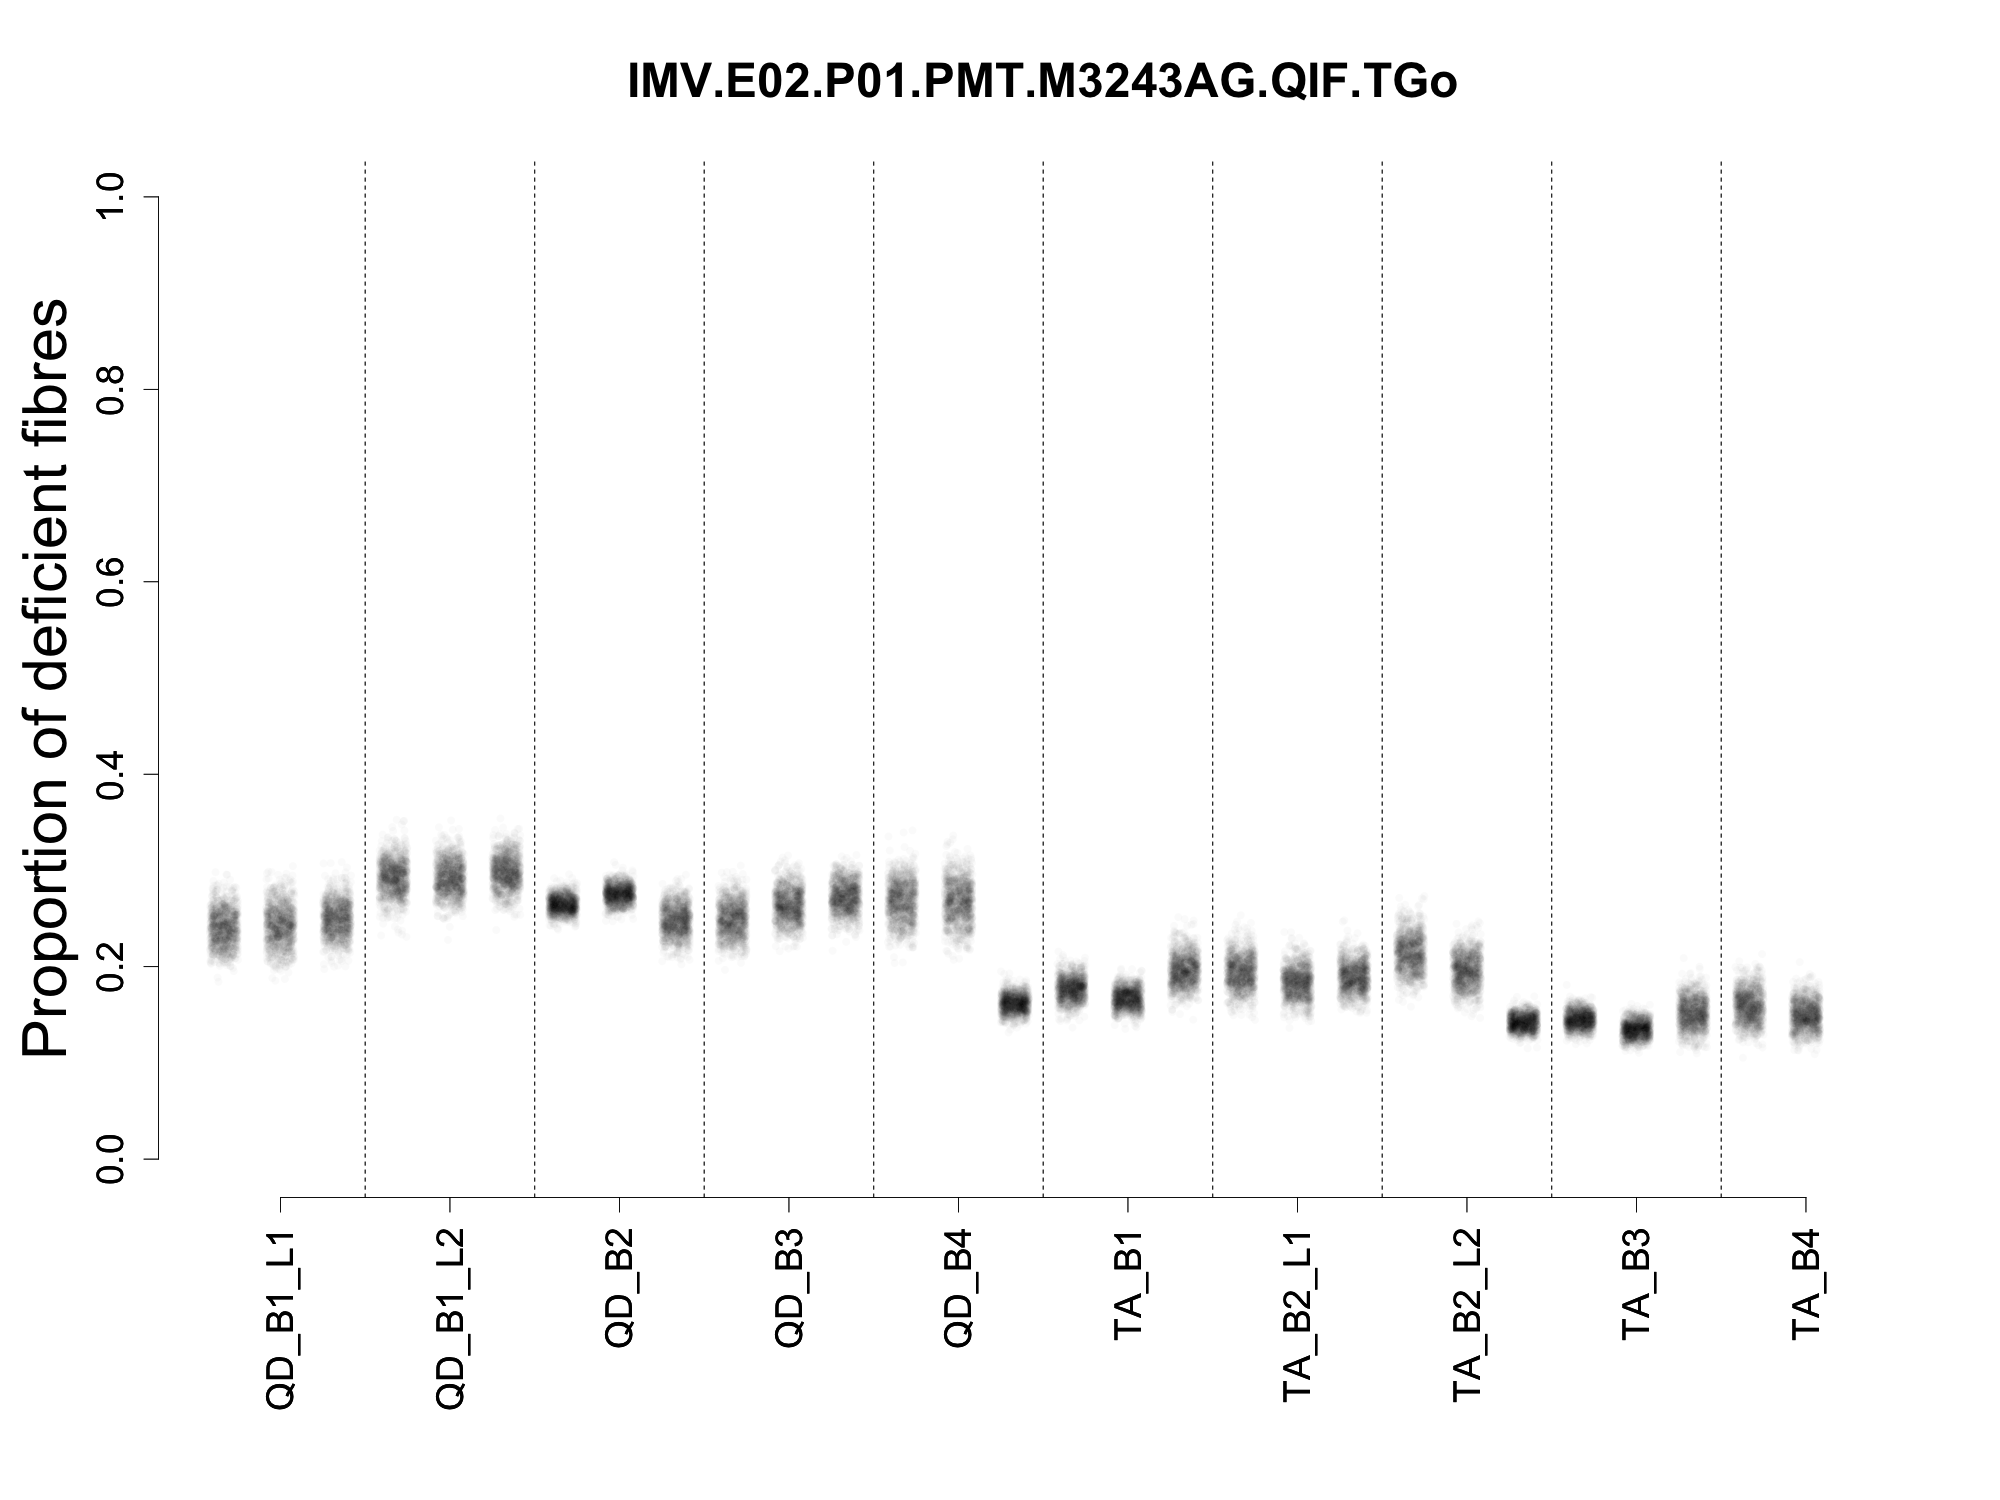
\includegraphics[width=0.5\textwidth]{bayes_prop.png}
    \caption{Proportion of deficient fibres from multiple samples of the same patient. }
    \label{fig:IMV}
\end{figure}



\end{document}
